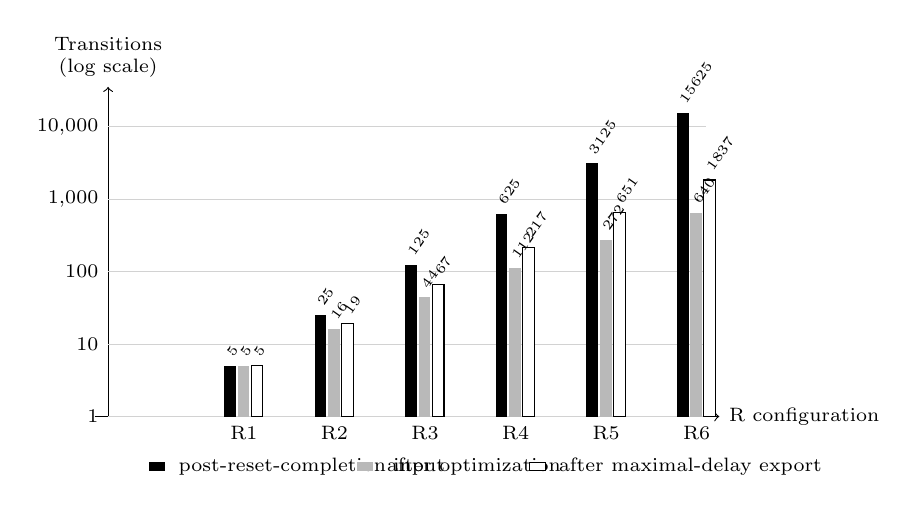
\begin{tikzpicture}[x=1.15cm,y=0.92cm,font=\scriptsize]
  % Vertical positions encode log10(edge count); the labelled y ticks are
  % 1, 10, 100, 1,000, and 10,000 transitions.
  \draw[->] (0.1,0) -- (7.0,0) node[right] {R configuration};
  \draw[->] (0.25,0) -- (0.25,4.55) node[above,align=center]
    {Transitions\\(log scale)};
  \foreach \y/\lab in {0/1,1/10,2/100,3/1{,}000,4/10{,}000} {
    \draw[gray!35] (0.25,\y) -- (6.85,\y);
    \node[left] at (0.25,\y) {\lab};
  }
  % Bars use log10(value) as height. Values above bars are exact counts.
  \foreach \x/\vin/\hin/\vopt/\hopt/\vexp/\hexp in {
    1/5/0.699/5/0.699/5/0.699,
    2/25/1.398/16/1.204/19/1.279,
    3/125/2.097/44/1.643/67/1.826,
    4/625/2.796/112/2.049/217/2.336,
    5/3125/3.494/272/2.435/651/2.814,
    6/15625/4.194/640/2.806/1837/3.264
  } {
    \pgfmathsetmacro{\xc}{\x+0.75}
    \pgfmathsetmacro{\xa}{\xc-0.22}
    \pgfmathsetmacro{\xb}{\xc-0.07}
    \pgfmathsetmacro{\xd}{\xc+0.08}
    \fill[black] (\xa,0) rectangle +(0.13,\hin);
    \fill[gray!55] (\xb,0) rectangle +(0.13,\hopt);
    \fill[white] (\xd,0) rectangle +(0.13,\hexp);
    \draw (\xd,0) rectangle +(0.13,\hexp);
    \node[rotate=55,anchor=west,font=\tiny] at (\xa,\hin+0.04) {\vin};
    \node[rotate=55,anchor=west,font=\tiny] at (\xb,\hopt+0.04) {\vopt};
    \node[rotate=55,anchor=west,font=\tiny] at (\xd,\hexp+0.04) {\vexp};
    \node[below] at (\xc,0) {R\x};
  }
  \fill[black] (0.7,-0.75) rectangle +(0.18,0.12);
  \node[right] at (0.92,-0.69) {post-reset-completion input};
  \fill[gray!55] (3.0,-0.75) rectangle +(0.18,0.12);
  \node[right] at (3.22,-0.69) {after optimization};
  \fill[white] (4.9,-0.75) rectangle +(0.18,0.12);
  \draw (4.9,-0.75) rectangle +(0.18,0.12);
  \node[right] at (5.12,-0.69) {after maximal-delay export};
\end{tikzpicture}
